Spatial signatures are unique as a classification method, limiting the potential
validation approaches. In this context, we focus on indirect methods that use ancillary datasets capturing
conceptually similar aspects of the environment. We compare the signatures with three of
such datasets, each focusing on a different classification perspective, but all related
to our classification to a degree when we can assume there will be a measurable level of
association between the two:

\begin{itemize}
    \item WorldPop settlement patterns of building footprints (2021)\cite{jochem2021tools}
    \item Classification of Multidimensional Open Data of Urban Morphology (MODUM) (2015)\cite{alexiou2016}
    \item Copernicus Urban Atlas (2018)\cite{eea2018}
\end{itemize}


\subsection*{Validation approach}
% General method of validation
    % data transfer (one or the other way depending on feasibility) chi-squared
    % statistic Cramer's V
All datasets, spatial signatures and those selected as validation contain a
categorical classification of space linked to their unique geometry. The first
requirement to be able to compare data products is to transfer their
information to the same geometry. We take two approaches for this step,
depending on the dataset we are comparing the signatures with:
an interpolation of one set of polygon-based data to another (input to ETCs);
or the conversion of
spatial signatures to the raster representation matching an input raster,
which is computationally more efficient when one of the layers is already a raster. The second
step is a statistical comparison of two sets of classification labels, one representing
spatial signature typology and the other validation classes. We use contingency tables
and Pearson's $\chi^{2}$ test to determine whether the frequencies of observed
(signature types) and expected (validation types) labels significantly differ in one or
more categories. Furthermore, we use Cramér's $V$ statistics\cite{cramer2016mathematical} to assess the strength of
the association.

\subsection*{WorldPop settlement patterns of building footprints}
% - WorldPop (Spsig)
    % description of dataset + figure
WorldPop settlement patterns of building footprints aim to derive a typology of
morphological patterns based on a gridded approach with cells of
100x100m, and building footprints. Authors measure six morphometric characters
linked to the grid cells and use them as input for an unsupervised clustering
algorithm leading to a six-class typology.
    % expectations regarding similarity
As the classification is dependent on building footprints, grid cells that do
not contain any information on the building-based pattern are treated as missing in the
final data product. For the validation of spatial signatures, this \textit{missing}
category is treated as a single class. It is assumed that the top-level large scale
patterns detected by the WorldPop method and spatial signatures will provide similar
results. However, there will be differences caused by the inclusion of function in spatial
signatures, higher granularity of both initial spatial units and the resulting
classification (6 vs 19 classes).

Signature typology is rasterized and linked to the WorldPop grid. The resulting
contingency table is shown in Figure \ref{fig:crosstab_worldpop}. There is a significant relationship between
two typologies, $\chi^{2} (114, N = 22993921) = 13341832, p < .001$. The strength of
association measured as Cram\'{e}r's $V$ is $0.311$, indicating moderate association.
    % results + contingency table figure

\begin{figure}
    \centering
    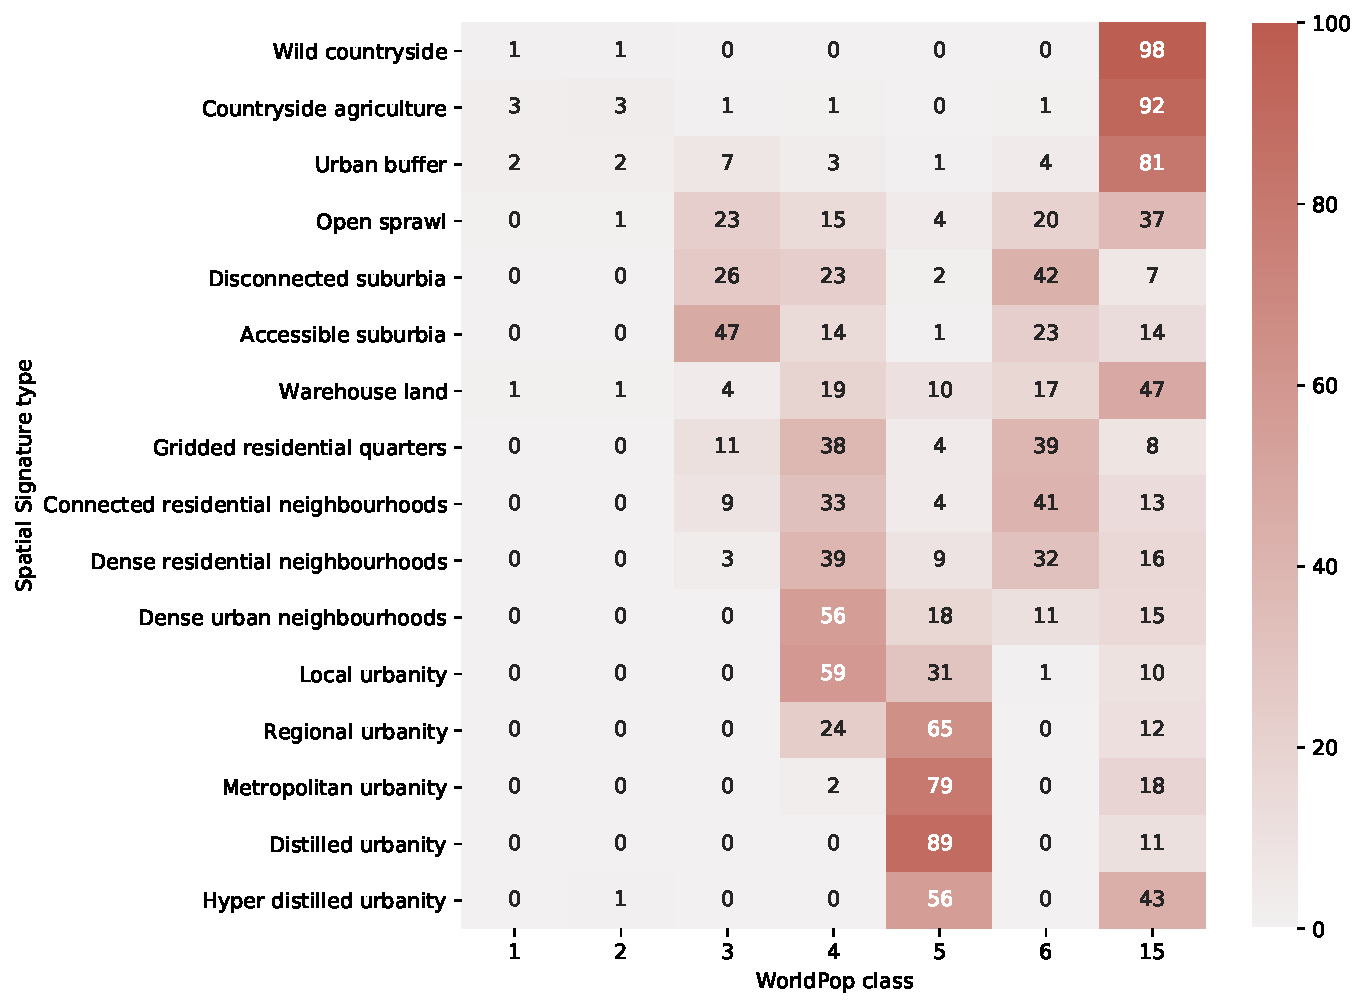
\includegraphics[width=.8\linewidth]{fig/crosstab_worldpop.pdf}
    \caption{Contingency table showing frequencies (in \%) of WorldPop classes within signature types.}
    \label{fig:crosstab_worldpop}
\end{figure}

\subsection*{MODUM}
% - MODUM (Spsig)
    % description of dataset + figure
Multidimensional Open Data Urban Morphology (MODUM) classification describes a typology
of neighbourhoods derived from 18 indicators capturing built environment as streets,
railways or parks, linked to the Census Output Area geometry. The classification
identifies 8 types of neighbourhoods.
    % expectations regarding similarity
Compared to the WorldPop classification, MODUM takes into account more features of
the built environment than building footprints, which makes it conceptually closer to the
spatial signatures. However, it is still focusing predominantly on the form component,
although there are some indicators that would be classified as function within the
signatures framework (e.g. population). The MODUM method uses a different way of
capturing context compared to the signatures, which leads to some classes being
determined predominantly by a single character. For example, the \textit{Railway Buzz} type
forms a narrow strip around the railway network, which is an effect signatures avoid.
    % results + contingency table figure
MODUM typology is available only for England and Wales. Therefore the validation takes
into account only ETCs covering the same area. The classification is linked to the
ETC geometry is based on the proportion (the type covering the largest portion of ETC is
assigned). The resulting contingency table is shown in Figure \ref{fig:crosstab_modum}. There is a
significant relationship between two typologies, $\chi^{2} (152, N = 13067584) =
13938867, p < .001$. The strength of association measured as Cramér's $V$ is $0.300$,
indicating moderate association of very similar levels we have seen above.

\begin{figure}
    \centering
    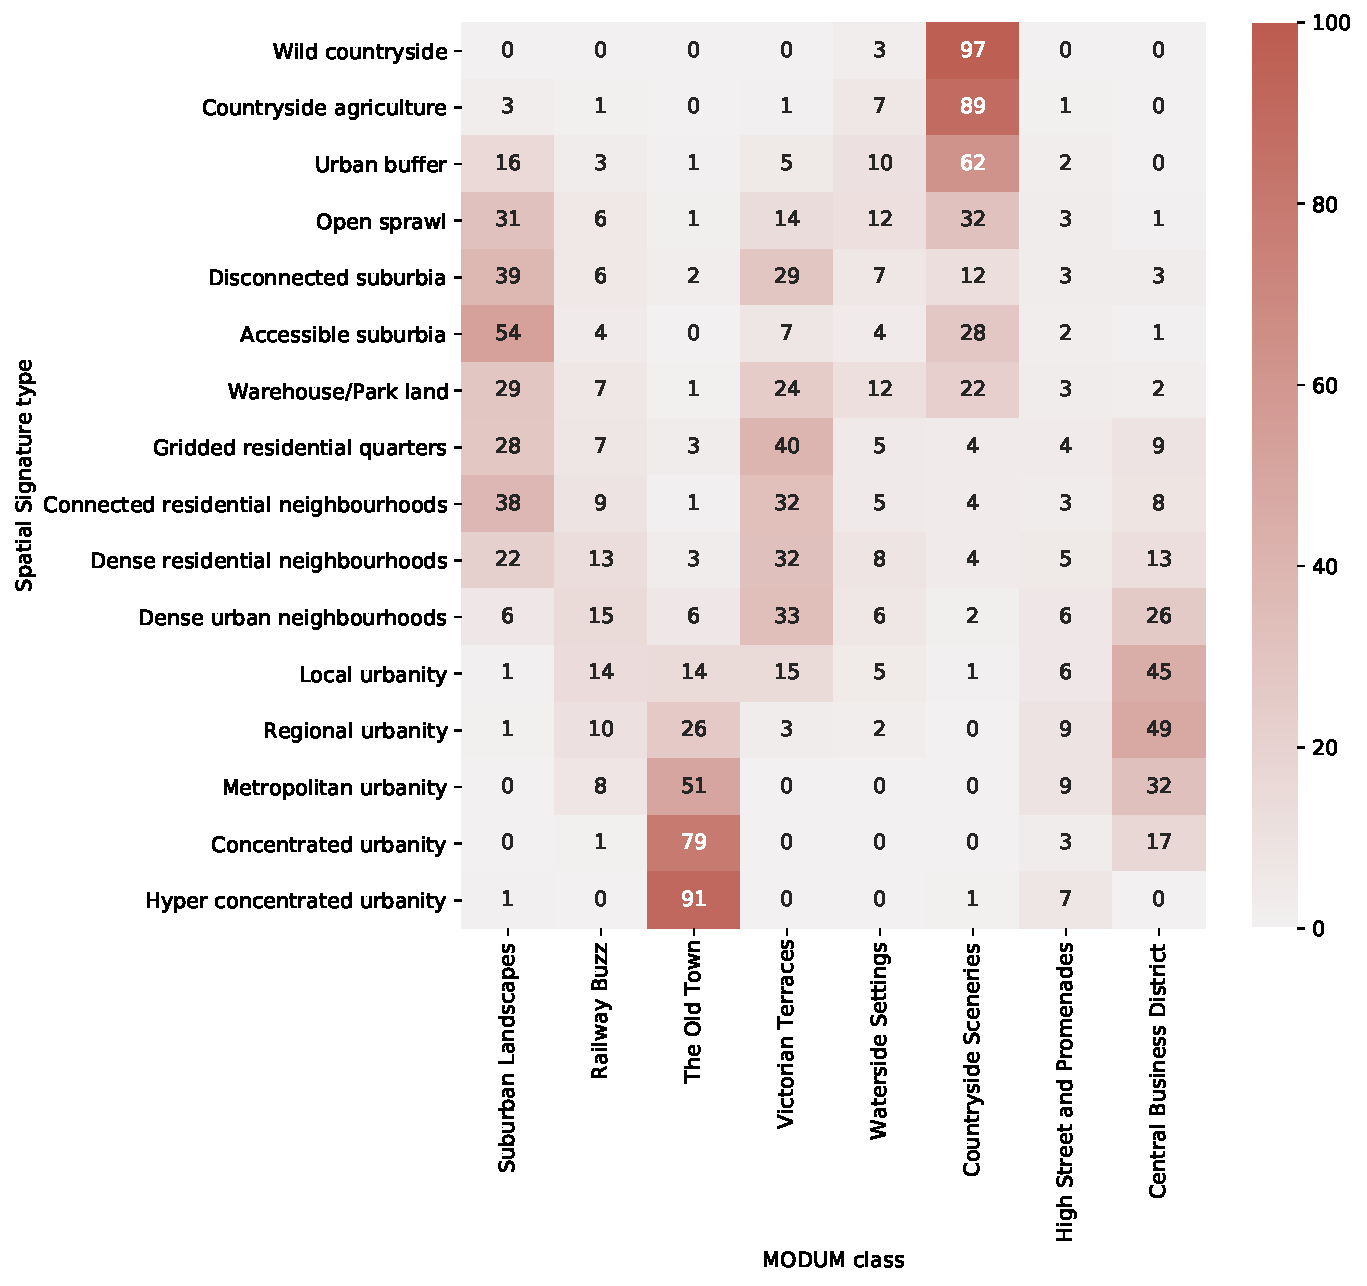
\includegraphics[width=.8\linewidth]{fig/crosstab_modum.pdf}
    \caption{Contingency table showing frequencies (in \%) of MODUM classes within signature types.}
    \label{fig:crosstab_modum}
\end{figure}

\subsection*{Copernicus Urban Atlas}
% - Urban atlas (Spsig)
    % description of dataset + figure
Copernicus Urban Atlas is the least similar of the validation datasets. It is a
high-resolution land use classification of functional urban areas derived primarily from
Earth Observation data enriched by other reference data as OpenStreetMap or topographic
maps. Its smallest spatial unit in urban areas is 0.25 ha and 1 ha in rural areas,
defined primarily by physical barriers. The Urban Atlas classification, which identifies
27 classes predefined classes using the supervised method.
    % expectations regarding similarity
The majority of urban areas is classified as urban fabric further distinguished based on
continuity and density resulting in six classes of the urban fabric. The classification does
not consider the type of the pattern or any other aspect. Furthermore, it does not take
into account what signatures call \textit{context} as each spatial unit is
classified independently, which in some cases leads to the high heterogeneity of
classification within a small portion of land. Signatures take a different approach.
Consequently, it is expected that the similarity between the two will be limited.
    % results + contingency table figure
Urban Atlas is available only for functional urban areas (FUA), leaving rural areas
unclassified. Validation then applies to FUAs only. The classification is linked to the
ETC geometry based on the proportion (the type covering the largest portion of ETC is
assigned). The resulting contingency table is shown in Figure \ref{fig:crosstab_ua}. There is a
significant relationship between two typologies, $\chi^{2} (450, N = 8396642) = 5229900,
p < .001$. The strength of association measured as Cramér's $V$ is $0.186$, indicating
a weak association.

\begin{figure}
    \centering
    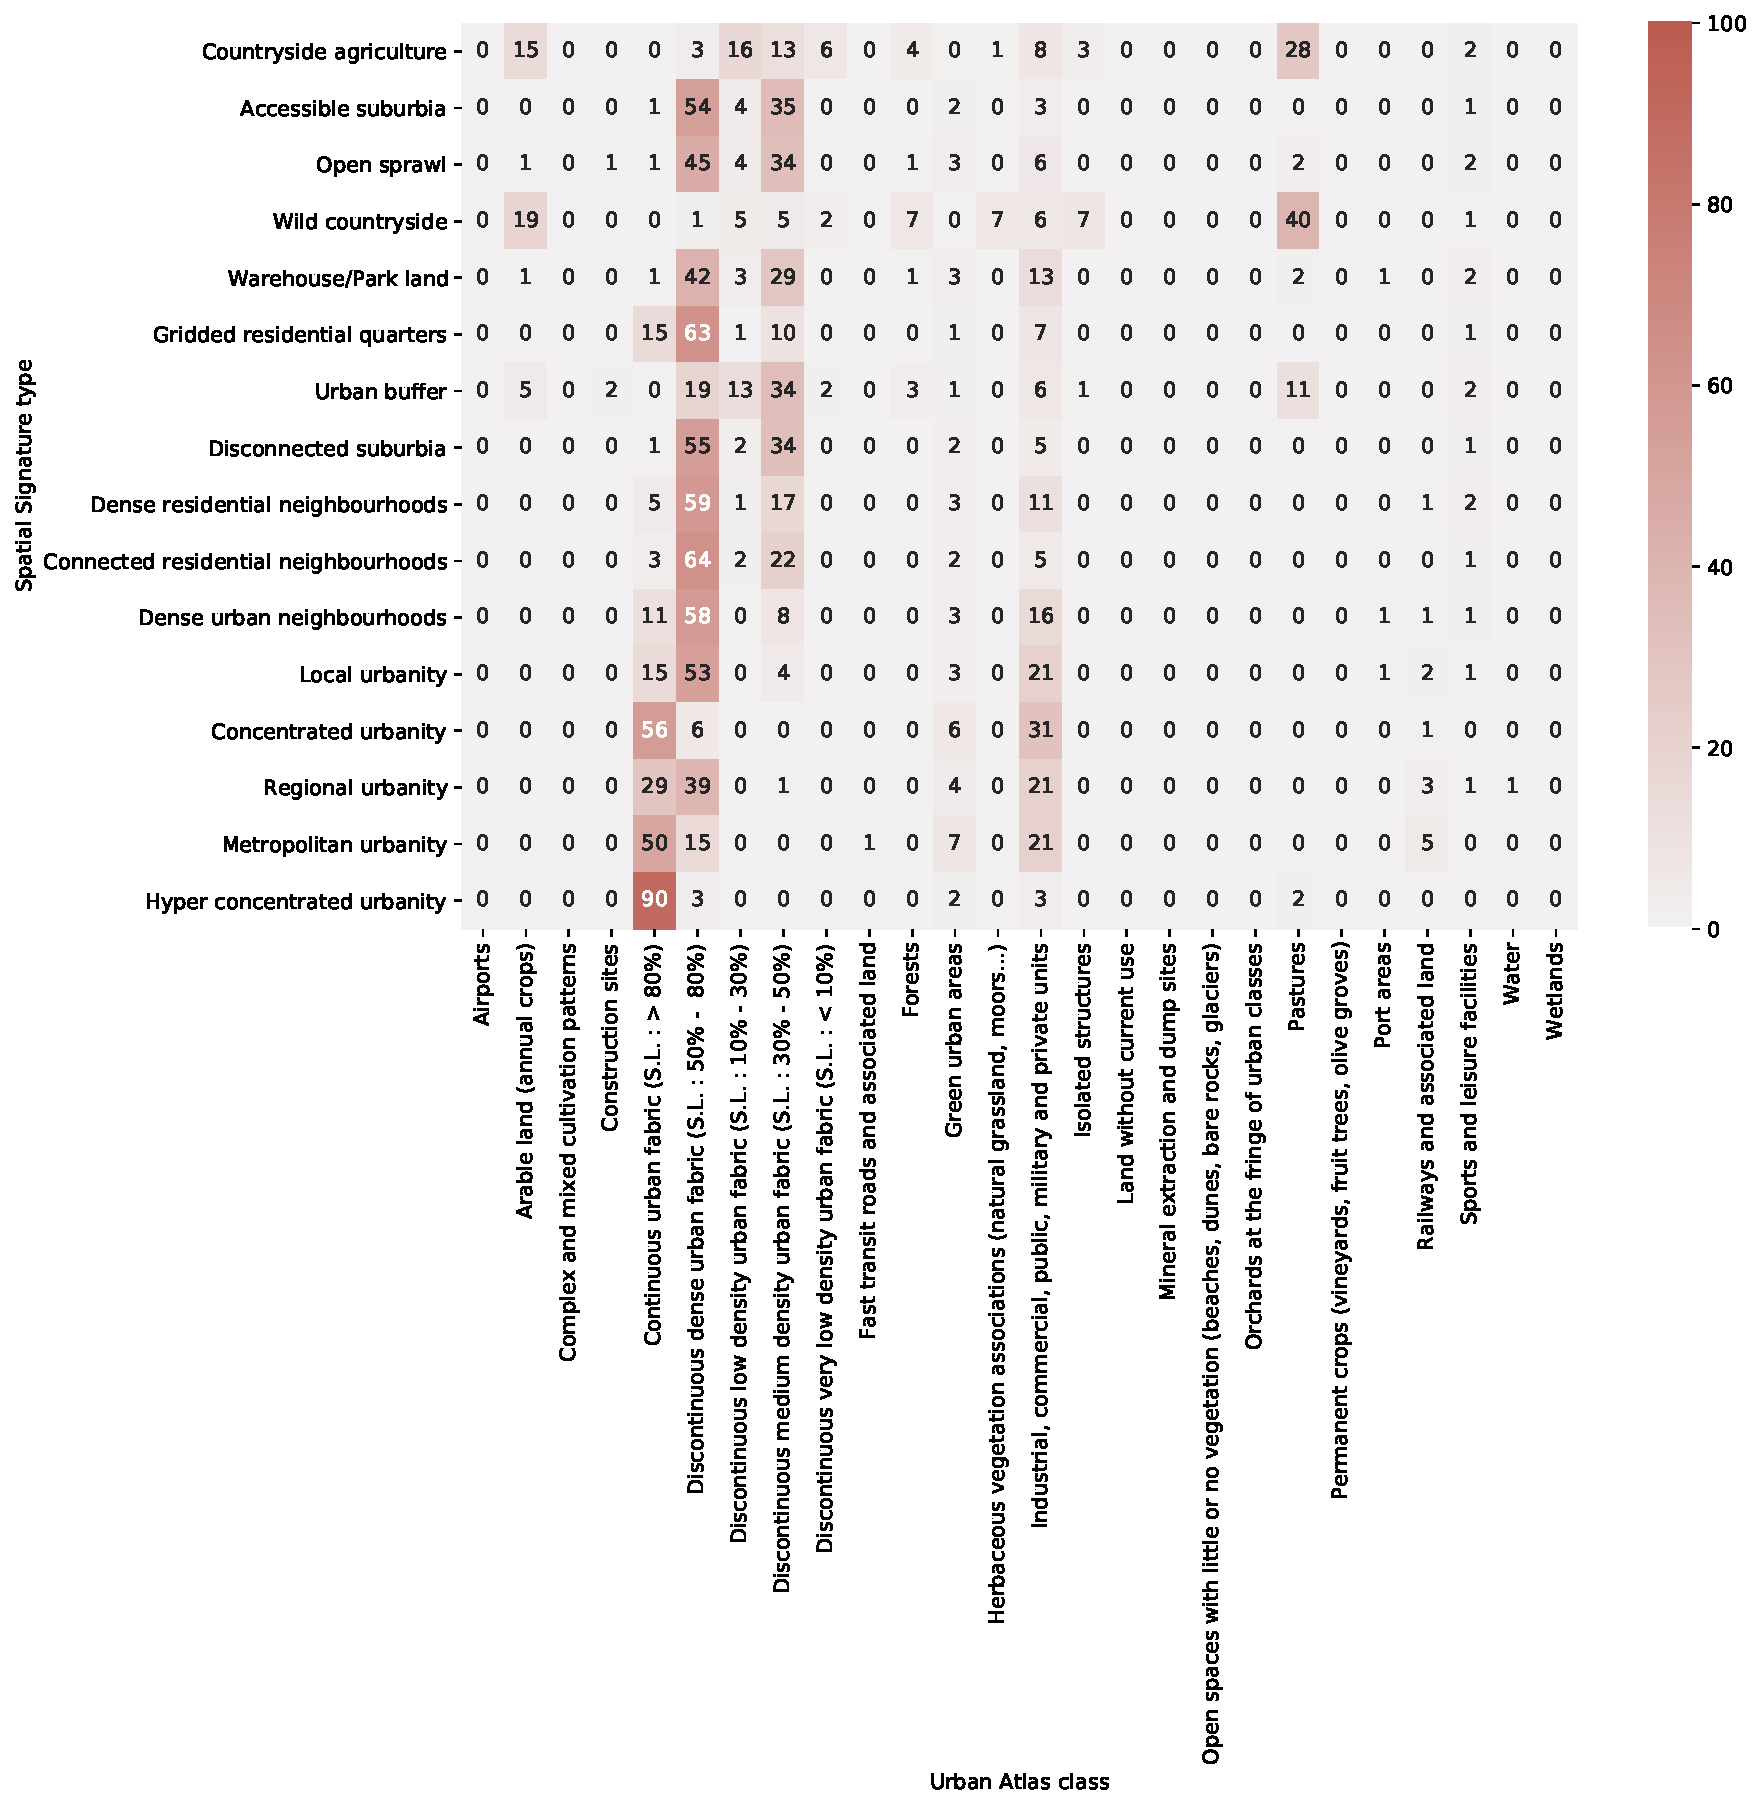
\includegraphics[width=\linewidth]{fig/crosstab_ua.pdf}
    \caption{Contingency table showing frequencies (in \%) of Urban Atlas classes within signature types.}
    \label{fig:crosstab_ua}
\end{figure}

\subsection*{Summary}
None of the comparisons shows more than a moderate association, but since none of the
validation datasets is aiming to capture the same conceptualization of space as spatial
signatures do, such a result is expected. The moderate association with both WorldPop
settlements patterns and MODUM is reassuring as both are conceptually closer to
signatures than the Urban Atlas (especially in their unsupervised design). Urban Atlas,
though very different in its aims and methods, still shows a measurable association,
which we interpret as sign that the key structural aspects forming cities are captured by both. The
validation exercise suggests that general patterns forming cities are shared among
signatures and existing typologies.

